% BeVietnam — pitch deck
% Style ported from ~/MyWorkspace/FactChecking/slide (CambridgeUS + UFT palette).
\documentclass[aspectratio=169, 10pt]{beamer}
\usepackage[utf8]{inputenc}
\usepackage[T1]{fontenc}
\usepackage[vietnamese]{babel}
\usepackage{bm}
\usepackage{tikz}
\usepackage{graphicx}
\usepackage{booktabs}
\usepackage{multirow}
\usepackage{amsmath}
\usepackage[most]{tcolorbox}
\usetikzlibrary{positioning, arrows.meta, calc, fit, backgrounds, shapes.geometric}

% ─── Theme (from FactChecking/slide/customize.tex) ────────────────────
\usetheme{CambridgeUS}
\definecolor{PROFMATgreen}{RGB}{0, 138, 163}
\definecolor{UFTgreen}{RGB}{0, 137, 124}
\definecolor{UFTblue}{RGB}{0, 84, 132}
\definecolor{UFTyellow}{RGB}{253, 185, 46}
\definecolor{UFTgray}{RGB}{132, 134, 136}

\setbeamertemplate{caption}[numbered]
\setbeamertemplate{itemize item}{\textcolor{UFTgreen}{\rule{1ex}{1ex}}}
\setbeamertemplate{itemize subitem}{\textcolor{UFTblue}{\rule{0.7ex}{0.7ex}}}
\setbeamercolor*{structure}{bg=UFTgreen,fg=black}
\setbeamercolor*{palette primary}{fg=black,bg=PROFMATgreen}
\setbeamercolor*{palette secondary}{fg=white,bg=UFTblue}
\setbeamercolor*{palette tertiary}{fg=black,bg=UFTgreen}
\setbeamercolor*{palette quaternary}{fg=white,bg=black}
\setbeamercolor{section in toc}{fg=black,bg=white}
\setbeamercolor{block title}{bg=UFTgreen,fg=white}
\setbeamercolor{block body}{bg=UFTgray!10,fg=black}
\setbeamercolor{titlelike}{fg=white, bg=UFTblue}
\setbeamercolor{frametitle}{bg=UFTgray!20,fg=UFTgreen}
\setbeamertemplate{navigation symbols}{}
\setbeamertemplate{blocks}[default]
\setbeamertemplate{background}{} % plain white (no bg image)

% footline (3 cols)
\setbeamercolor{author in head/foot}{bg=UFTgreen, fg=black}
\setbeamercolor{title  in head/foot}{bg=UFTblue,  fg=white}
\setbeamercolor{date   in head/foot}{bg=UFTgreen, fg=black}
\setbeamerfont{author in head/foot}{size=\footnotesize}
\setbeamerfont{title  in head/foot}{size=\footnotesize}
\setbeamerfont{date   in head/foot}{size=\footnotesize}
\setbeamertemplate{footline}{%
  \leavevmode
  \hbox{%
    \begin{beamercolorbox}[wd=.33\paperwidth,ht=2.5ex,dp=1.1ex,center]{author in head/foot}%
      \hspace*{1ex}\insertshortauthor
    \end{beamercolorbox}%
    \begin{beamercolorbox}[wd=.47\paperwidth,ht=2.5ex,dp=1.1ex,center]{title in head/foot}%
      \parbox{\dimexpr.45\paperwidth\relax}{\centering\insertshorttitle}%
    \end{beamercolorbox}%
    \begin{beamercolorbox}[wd=.20\paperwidth,ht=2.5ex,dp=1.1ex,center]{date in head/foot}%
      \hspace{4ex}\insertframenumber{} / \inserttotalframenumber\hspace{1ex}%
    \end{beamercolorbox}%
  }%
  \vskip0pt%
}
\setbeamersize{text margin left=0.8cm, text margin right=0.8cm}

% ─── helpers ──────────────────────────────────────────────────────────
\newtcbox{\kw}{on line, arc=3pt, colback=UFTgreen!12, colframe=UFTgreen!55,
  boxrule=0.6pt, boxsep=1pt, left=4pt, right=4pt, top=2pt, bottom=2pt}
\newtcolorbox{card}[1]{colback=UFTgray!8, colframe=UFTgreen, fonttitle=\bfseries\small,
  title=#1, boxrule=0.6pt, arc=3pt, left=3pt, right=3pt, top=2pt, bottom=2pt}
% photo tile with graceful fallback if image missing
\newcommand{\phototile}[3]{% path, width, caption
  \begin{tikzpicture}
  \node[inner sep=0pt] (im) {%
    \IfFileExists{#1}{\includegraphics[width=#2]{#1}}{%
      \fcolorbox{UFTgray!50}{UFTgray!12}{\parbox[c][2.3cm][c]{#2}{\centering\scriptsize\itshape\color{UFTgray}[ảnh]\par\tiny thêm vào img/}}}};
  \node[below=1pt of im, font=\scriptsize\color{UFTblue}] {#3};
  \end{tikzpicture}}
% mobile screenshot tile (defined at top level to avoid pgf \iterate clash)
\newcommand{\mobshot}[2]{\IfFileExists{../report/images/#1}{\includegraphics[height=0.62\textheight]{../report/images/#1}}{\fcolorbox{UFTgray!50}{UFTgray!12}{\parbox[c][3.5cm][c]{2.2cm}{\centering\scriptsize\itshape\color{UFTgray}#2}}}}

% tikz styles for pipeline
\tikzset{
  comp/.style={rectangle, rounded corners, draw=UFTblue!70, fill=white,
    minimum height=7mm, minimum width=20mm, align=center, inner sep=2pt, font=\scriptsize},
  store/.style={comp, fill=UFTgray!12},
  ext/.style={comp, draw=UFTyellow!80!black, dashed, fill=UFTyellow!12},
  llm/.style={comp, fill=UFTgreen!14, minimum width=30mm},
  flow/.style={-{Latex[length=2mm]}, thick, UFTblue!70},
  ret/.style={-{Latex[length=2mm]}, thick, dashed, UFTgray},
}

\title[BeVietnam]{\textbf{BeVietnam}\\\large Hệ thống Du lịch Thông minh dựa trên AI Agent}
\author[Nhóm BeVietnam]{Nhóm BeVietnam}
\institute[HCMUS]{Trường ĐH Khoa học Tự nhiên --- ĐHQG-HCM\\Khoa Công nghệ Thông tin}
\date{}

\begin{document}

% ── Slide 1: Title ───────────────────────────────────────────────────
\begin{frame}[plain]
  \titlepage
  \begin{center}\footnotesize\color{UFTgray}
  Pilot: Huế \quad|\quad Web (Azure) + Mobile (Android) + AI Core + vLLM
  \end{center}
\end{frame}

% ── Slide 2: Pain Points ─────────────────────────────────────────────
\begin{frame}{Pain Points --- vấn đề nhóm giải quyết}
  \begin{columns}[T]
  \column{0.33\textwidth}\centering
    \phototile{img/pain_scattered.png}{\linewidth}{Thông tin phân tán}
    \kw{Google Maps + blog + TikTok}\\[2pt]
    \scriptsize Du khách phải mở nhiều nguồn rời rạc.
  \column{0.33\textwidth}\centering
    \phototile{img/pain_return.jpg}{\linewidth}{Tỷ lệ quay lại thấp}
    \kw{VN 10--40\%} \kw{Thái Lan $\sim$80\%}\\[2pt]
    \scriptsize Thiếu lý do để quay lại lần hai.
  \column{0.33\textwidth}\centering
    \phototile{img/pain_passive.jpg}{\linewidth}{Trải nghiệm thụ động}
    \kw{Đến rồi không biết làm gì}\\[2pt]
    \scriptsize Thiếu chiều sâu văn hóa tại điểm đến.
  \end{columns}
  \vfill
  \begin{center}\small
  \kw{21,2 triệu khách quốc tế 2025} nhưng \kw{tỷ lệ quay lại thấp} $\Rightarrow$ bài toán \textbf{giữ chân}.
  \end{center}
\end{frame}

% ── Slide 3: Proposed Solution ───────────────────────────────────────
\begin{frame}{Giải pháp đề xuất}
  \begin{center}\large
  Một ứng dụng gộp \textbf{khám phá $\to$ gợi ý $\to$ trải nghiệm $\to$ xác minh}.
  \end{center}
  \vspace{2mm}
  \begin{center}
  \resizebox{0.95\textwidth}{!}{%
  \begin{tikzpicture}[node distance=6mm]
    \node[comp, fill=UFTgreen!12] (a) {Curated\\Place Discovery};
    \node[comp, fill=UFTgreen!12, right=of a] (b) {Dynamic\\Recommendation};
    \node[comp, fill=UFTgreen!12, right=of b] (c) {Storyline\\Mission Path};
    \node[comp, fill=UFTgreen!12, right=of c] (d) {Vision Capture\\Verification};
    \draw[flow] (a)--(b); \draw[flow] (b)--(c); \draw[flow] (c)--(d);
    \node[below=1pt of a, font=\scriptsize\color{UFTgray}] {dữ liệu nền};
    \node[below=1pt of b, font=\scriptsize\color{UFTgray}] {nên đi đâu lúc này};
    \node[below=1pt of c, font=\scriptsize\color{UFTgray}] {đến đó làm gì};
    \node[below=1pt of d, font=\scriptsize\color{UFTgray}] {nối số $\to$ thực địa};
  \end{tikzpicture}}
  \end{center}
  \vfill
  \begin{columns}
  \column{0.5\textwidth}
    \kw{Gợi ý theo ngữ cảnh thời gian thực}\\[3pt]
    \kw{Giải thích được (explainable ranking)}
  \column{0.5\textwidth}
    \kw{Học văn hóa gắn hành động thực địa}\\[3pt]
    \kw{Xác minh ảnh bằng VLM tự host}
  \end{columns}
\end{frame}

% ── Slide 4: Problem Analysis ────────────────────────────────────────
\begin{frame}{Phân tích bài toán --- 5W1H \& 5 Whys}
  \begin{columns}[T]
  \column{0.52\textwidth}
  \footnotesize
  \begin{tabular}{@{}ll@{}}
  \textbf{What} & Giữ chân du khách bằng trải nghiệm văn hóa \\
  \textbf{Why}  & Tỷ lệ quay lại thấp, thông tin phân tán \\
  \textbf{Who}  & Du khách nội địa + quốc tế (pilot Huế) \\
  \textbf{Where}& Web + Mobile, dữ liệu quanh vị trí \\
  \textbf{When} & Theo bối cảnh: thời tiết, thời điểm \\
  \textbf{How}  & AI Core + backend + VLM xác minh \\
  \end{tabular}
  \column{0.46\textwidth}
  \scriptsize \textbf{5 Whys (chuỗi gốc rễ):}
  \begin{tikzpicture}[node distance=2.2mm and 0mm, every node/.style={font=\scriptsize}]
    \node[comp, fill=UFTyellow!15] (q1) {Không quay lại};
    \node[comp, fill=UFTyellow!15, below=of q1] (q2) {Trải nghiệm nông};
    \node[comp, fill=UFTyellow!15, below=of q2] (q3) {Không biết làm gì tại chỗ};
    \node[comp, fill=UFTyellow!15, below=of q3] (q4) {Thiếu dẫn dắt văn hóa};
    \node[comp, fill=UFTgreen!15, below=of q4] (q5) {$\Rightarrow$ Storyline + Capture};
    \draw[flow] (q1)--(q2);\draw[flow] (q2)--(q3);\draw[flow] (q3)--(q4);\draw[flow] (q4)--(q5);
  \end{tikzpicture}
  \end{columns}
\end{frame}

% ── Slide 5: Decomposition ───────────────────────────────────────────
\begin{frame}{Decomposition --- chia bài toán $\to$ dữ liệu}
  \begin{center}
  \resizebox{0.96\textwidth}{!}{%
  \begin{tikzpicture}[level distance=12mm, sibling distance=30mm,
    every node/.style={comp, font=\scriptsize}, edge from parent/.style={flow, draw}]
    \node[fill=UFTblue!12] {Bài toán du lịch}
      child {node {Khám phá} child {node[store] {Place}}}
      child {node {Gợi ý ngữ cảnh} child {node[store] {Post + tags}}}
      child {node {Hiểu tại chỗ} child {node[store] {Question Pool}}}
      child {node {Xác minh} child {node[store] {Capture}}};
  \end{tikzpicture}}
  \end{center}
  \vfill
  \begin{center}\small
  Mỗi lát cắt nghiệp vụ $\Rightarrow$ một thực thể dữ liệu rõ ràng (schema thống nhất).
  \end{center}
\end{frame}

% ── Slide 6: Architecture Overview (main diagram) ────────────────────
\begin{frame}{Tổng quan kiến trúc --- 3 lớp}
  \begin{center}
  \resizebox{0.92\textwidth}{!}{%
  \begin{tikzpicture}
    % frontend
    \node[comp] (web) {Web\\(Azure)};
    \node[comp, right=10mm of web] (mob) {Mobile\\(Android)};
    % backend
    \node[comp, below=14mm of web] (nearby) {/places\\/nearby};
    \node[comp, right=5mm of nearby] (feed) {/feed};
    \node[comp, right=5mm of feed] (pool) {/question\\-pool};
    \node[comp, right=5mm of pool] (verify) {/verify\\-capture};
    \node[store, below=6mm of feed] (pg) {PostgreSQL};
    \node[store, right=5mm of pg] (minio) {MinIO};
    \node[ext, left=10mm of nearby] (fsq) {Foursquare};
    \node[ext, above=3mm of fsq] (ow) {OpenWeather};
    \node[ext, below=3mm of fsq] (serp) {SerpAPI};
    % vllm
    \node[llm, below=24mm of verify] (vllm) {Qwen2.5-VL-7B\\(vLLM, L40)};
    \begin{scope}[on background layer]
      \node[draw=UFTgray!40, fill=UFTblue!4, rounded corners, fit=(web)(mob), inner sep=3mm] (Lf){};
      \node[draw=UFTgray!40, fill=UFTgreen!5, rounded corners, fit=(nearby)(verify)(pg)(minio)(ow)(serp), inner sep=3mm] (Lb){};
      \node[draw=UFTgray!40, fill=UFTyellow!6, rounded corners, fit=(vllm), inner sep=3mm] (Lv){};
    \end{scope}
    \node[rotate=90, font=\scriptsize\bfseries, anchor=south] at ([xshift=-2mm]Lf.west) {Frontend};
    \node[rotate=90, font=\scriptsize\bfseries, anchor=south] at ([xshift=-2mm]Lb.west) {Backend};
    \node[rotate=90, font=\scriptsize\bfseries, anchor=south] at ([xshift=-2mm]Lv.west) {vLLM};
    \draw[flow] (web.south) -- ([yshift=3mm]web.south|-Lb.north) node[midway,right,font=\tiny]{REST};
    \draw[flow] (mob.south) -- ([yshift=3mm]mob.south|-Lb.north);
    \draw[flow] (nearby)--(fsq); \draw[flow] (nearby.west) to[bend left=12] (ow.east);
    \draw[flow] (verify.south west) to[out=200,in=0] (serp.east);
    \draw[flow] (feed)--(pg); \draw[flow] (verify)--(minio);
    \draw[flow] (verify.south)--(vllm.north) node[midway,right,font=\tiny]{ảnh+rubric};
    \draw[ret] ([xshift=5mm]vllm.north)--([xshift=5mm]verify.south) node[midway,right,font=\tiny]{0--1};
  \end{tikzpicture}}
  \end{center}
  \begin{center}\scriptsize
  Backend giữ product state; nguồn ngoài khóa sau backend; \textbf{chỉ} /verify-capture chạm vLLM.
  \end{center}
\end{frame}

% ── Slide 6b: Offline knowledge pipeline ─────────────────────────────
\begin{frame}{Pipeline sinh tri thức (offline)}
  \begin{center}
  \resizebox{0.97\textwidth}{!}{%
  \begin{tikzpicture}[node distance=7mm]
    \node[store] (books) {Sách OCR\\(.md)};
    \node[comp, right=of books] (chunk) {Section-aware\\chunker};
    \node[llm, right=of chunk] (vllm) {vLLM LLM\\(grounded JSON)};
    \node[comp, right=of vllm, yshift=7mm, fill=UFTblue!10] (ck) {hue\_book\_chunks};
    \node[comp, right=of vllm, yshift=-7mm, fill=UFTblue!10] (qp) {question\_pool\\+ spotlights};
    \node[comp, below=9mm of vllm, fill=UFTyellow!18] (rev) {Human review\\needs\_review$\to$approved};
    \draw[flow] (books)--(chunk); \draw[flow] (chunk)--(vllm);
    \draw[flow] (vllm)--(ck); \draw[flow] (vllm)-- node[below,font=\tiny,pos=.6]{per-landmark} (qp);
    \draw[flow] (ck)|-(rev); \draw[flow] (qp)|-(rev);
  \end{tikzpicture}}
  \end{center}
  \vspace{1mm}
  \begin{center}\scriptsize
  \kw{vLLM tự host thay Gemini 429} \quad \kw{grounded + needs\_review} \quad \kw{sinh sẵn offline $\Rightarrow$ runtime nhẹ}\\[3pt]
  Cùng L40: \textbf{offline} = LLM sinh nội dung \quad|\quad \textbf{runtime} = VLM chấm ảnh.
  \end{center}
\end{frame}

% ── Slide 7: Core Features ───────────────────────────────────────────
\begin{frame}{Core Features (pilot Huế)}
  \begin{columns}[T]
  \column{0.5\textwidth}
    \begin{card}{Curated Place Discovery}\scriptsize Dữ liệu điểm đến chọn lọc + nguồn gốc.\end{card}\vspace{2pt}
    \begin{card}{Dynamic Recommendation Feed}\scriptsize Xếp hạng theo ngữ cảnh + giải thích.\end{card}\vspace{2pt}
    \begin{card}{Realtime Bubble Map}\scriptsize POI Foursquare 3km + thời tiết.\end{card}
  \column{0.5\textwidth}
    \begin{card}{Storyline Mission Path}\scriptsize Lộ trình kiểu Duolingo từ question pool.\end{card}\vspace{2pt}
    \begin{card}{Vision Capture Verification}\scriptsize VLM chấm ảnh theo rubric.\end{card}\vspace{2pt}
    \begin{card}{Bilingual Experience}\scriptsize Việt + Anh trong cùng bản ghi.\end{card}
  \end{columns}
\end{frame}

% ── Slide 8: Ranking algorithm ───────────────────────────────────────
\begin{frame}{Explainable Ranking --- công thức điểm}
  \begin{center}
  \small
  $\text{score}(p) = b + (\alpha+\beta\,|I\cap C_p|)\cdot\mathbf{1}[\text{match}] + f_w + f_t + f_s - \gamma\cdot\mathbf{1}[p\in V]$
  \end{center}
  \vspace{1mm}
  \begin{columns}[T]
  \column{0.5\textwidth}\scriptsize
  \kw{$b=5$} cơ sở \quad \kw{$\alpha=10,\beta=5$} sở thích\\[3pt]
  \kw{$f_w\in\{20,6,0\}$} thời tiết\\[3pt]
  \kw{$f_t\in\{12,4,0\}$} thời điểm \quad \kw{$f_s\in\{8,0\}$} mùa\\[3pt]
  \kw{$\gamma=25$} phạt nơi đã ghé
  \column{0.5\textwidth}\scriptsize
  Chuẩn hóa: $\text{clip}(\text{score}/60,\,0,\,1)$\\[4pt]
  \textbf{Mỗi factor score được trả về} $\Rightarrow$ giải thích vì sao điểm được nâng/hạ.\\[4pt]
  \textit{Hạn chế:} traffic/crowd hiện mô phỏng + fallback.
  \end{columns}
\end{frame}

% ── Slide 9: Bubble Map ──────────────────────────────────────────────
\begin{frame}{Realtime Bubble Map}
  \begin{center}
    \IfFileExists{../report/images/bevietnam_map.png}
      {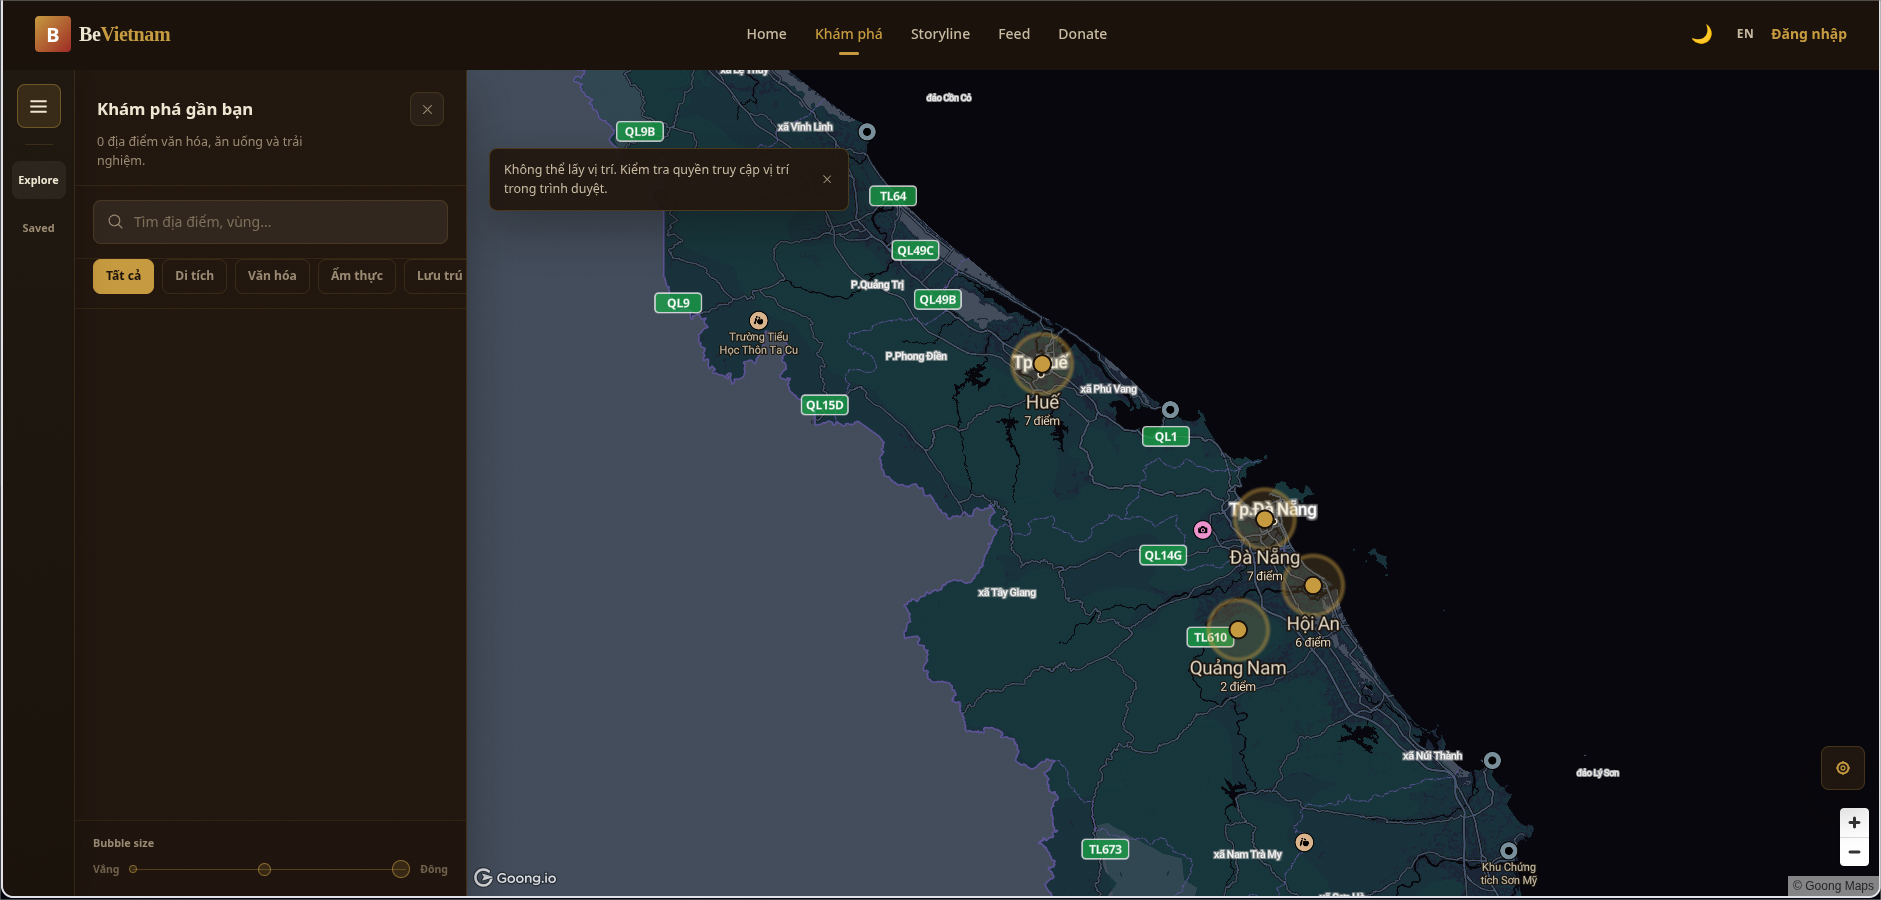
\includegraphics[width=0.48\textwidth,height=0.52\textheight,keepaspectratio]{../report/images/bevietnam_map.png}}
      {\fcolorbox{UFTgray!50}{UFTgray!12}{\parbox[c][2.6cm][c]{0.48\textwidth}{\centering\scriptsize\itshape\color{UFTgray}bevietnam\_map.png}}}\hfill
    \IfFileExists{../report/images/bevietnam_detail_map.png}
      {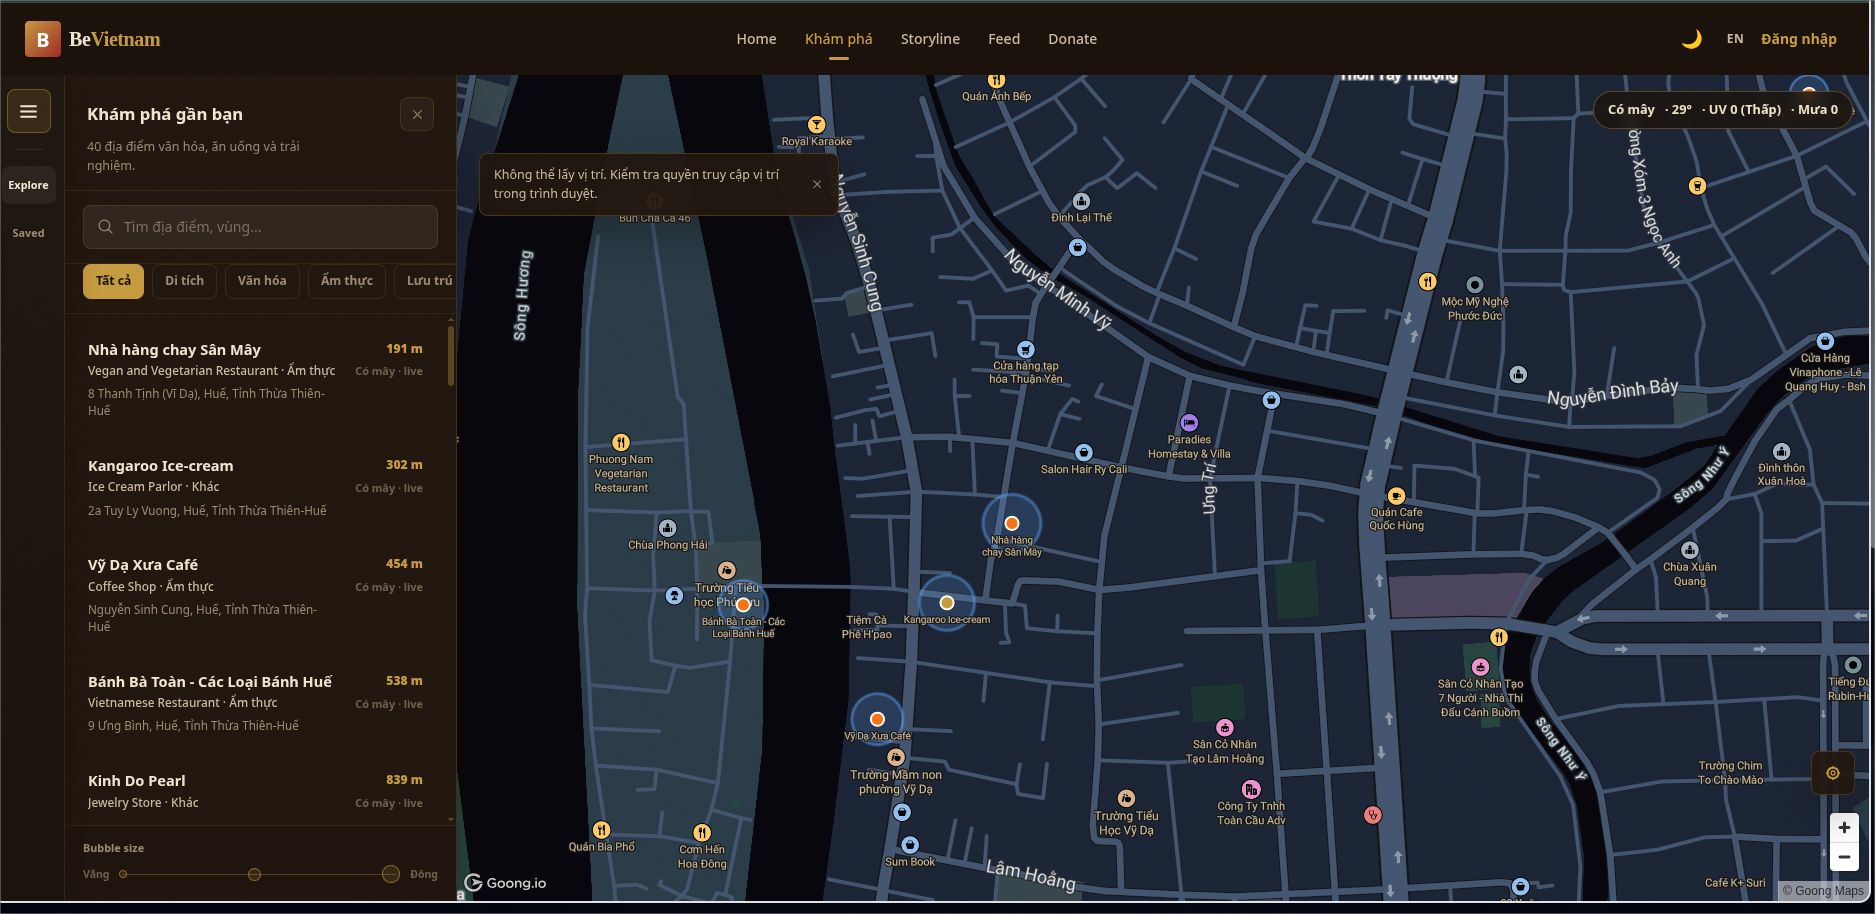
\includegraphics[width=0.48\textwidth,height=0.52\textheight,keepaspectratio]{../report/images/bevietnam_detail_map.png}}
      {\fcolorbox{UFTgray!50}{UFTgray!12}{\parbox[c][2.6cm][c]{0.48\textwidth}{\centering\scriptsize\itshape\color{UFTgray}bevietnam\_detail\_map.png}}}\\[1pt]
    {\scriptsize\color{UFTblue} Tổng quan \hspace{0.32\textwidth} Chi tiết một địa điểm}
  \end{center}
  \vspace{1mm}
  \begin{center}\scriptsize
    \kw{GPS thực + 3km} \quad \kw{POI Foursquare} \quad \kw{thời tiết OpenWeather} \quad \kw{co giãn theo khoảng cách (haversine)}\\[3pt]
    Web + Mobile dùng chung \texttt{/places/nearby} $\Rightarrow$ nhất quán. \textit{Khóa API ở backend.}
  \end{center}
\end{frame}

% ── Slide 10: Storyline ──────────────────────────────────────────────
\begin{frame}{Storyline Mission Path}
  \begin{columns}[T]
  \column{0.5\textwidth}
  \begin{center}
  \IfFileExists{../report/images/storyline.png}
    {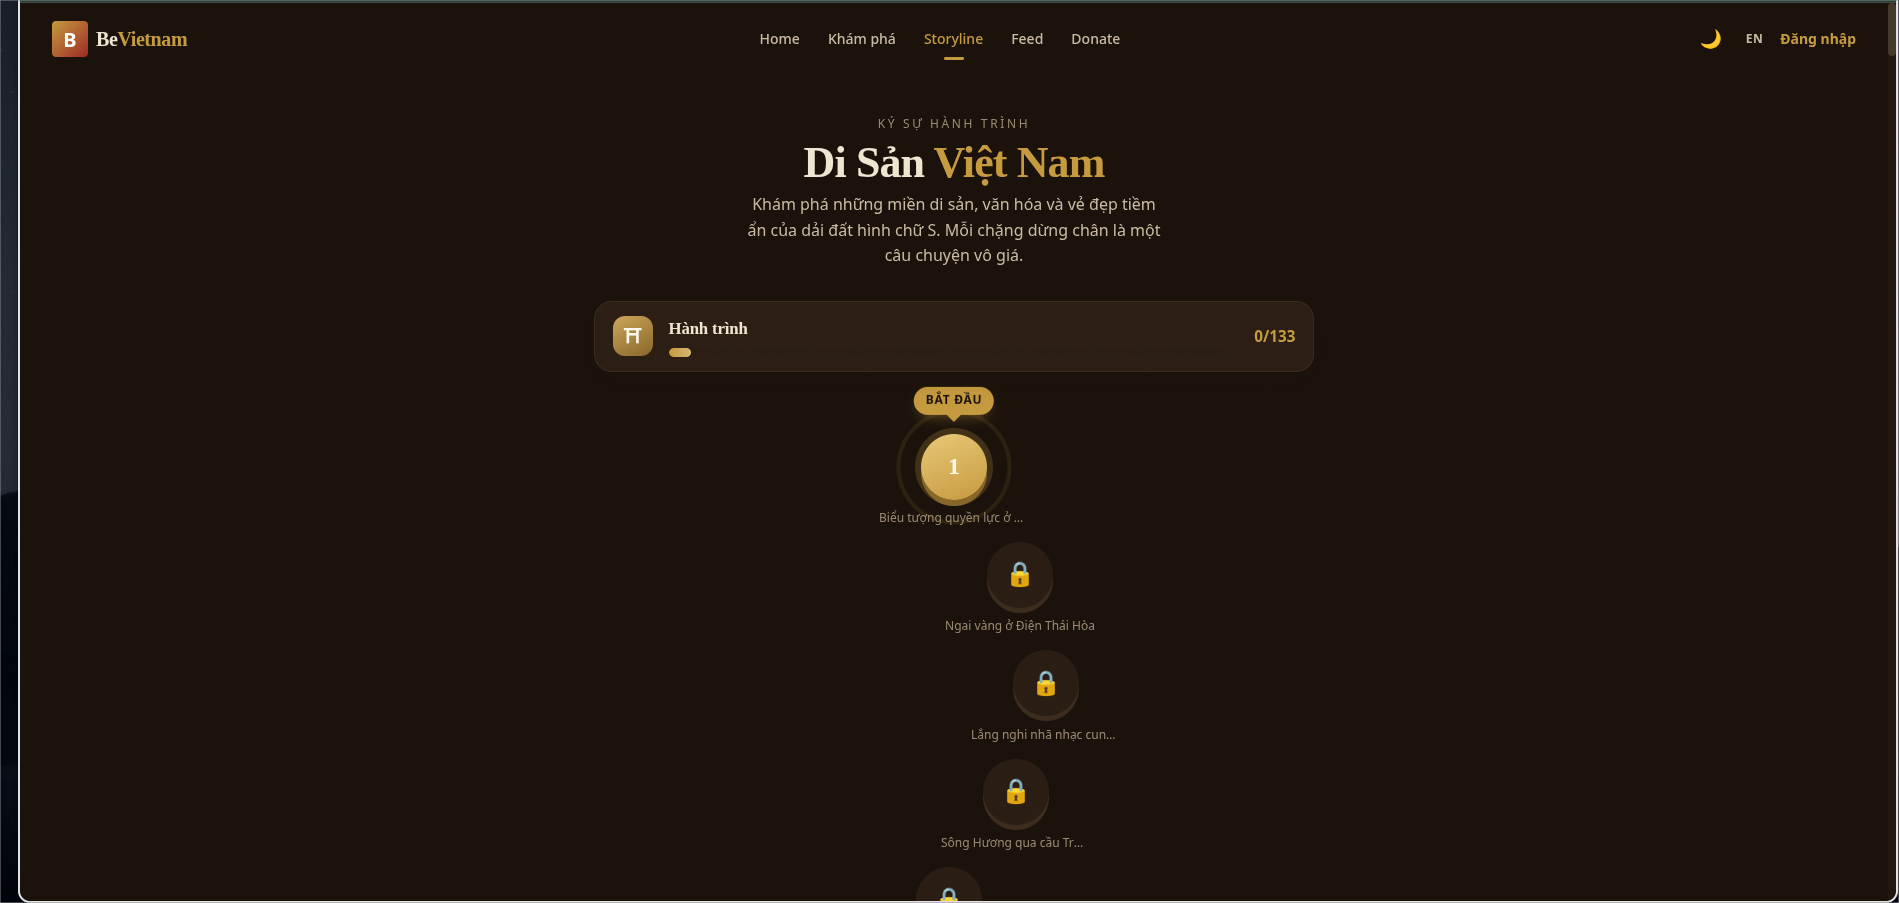
\includegraphics[width=\linewidth,height=0.62\textheight,keepaspectratio]{../report/images/storyline.png}}
    {\fcolorbox{UFTgray!50}{UFTgray!12}{\parbox[c][3cm][c]{\linewidth}{\centering\scriptsize\itshape\color{UFTgray}storyline.png}}}
  \end{center}
  \scriptsize Lộ trình kiểu Duolingo, mở khóa tuần tự.
  \column{0.5\textwidth}\scriptsize
  Nội dung \textbf{sinh trước offline} vào question pool:
  \begin{tcolorbox}[colback=UFTgray!8, colframe=UFTgreen, boxrule=0.5pt, arc=2pt, fontupper=\ttfamily\tiny]
\{ "question\_id": "hue-imperial-01-ngo-mon",\\
\ "title": "Bieu tuong quyen luc o Ngo Mon",\\
\ "latitude": 16.4699, "radius\_meters": 600,\\
\ "required\_media": "photo",\\
\ "metadata": \{ "step\_index": 1, "total\_steps": 3 \} \}
  \end{tcolorbox}
  Runtime: client nạp pool $\to$ dựng path $\to$ quản lý unlock.
  \end{columns}
\end{frame}

% ── Slide 11: Capture Verification ───────────────────────────────────
\begin{frame}{Vision Capture Verification}
  \begin{center}
  \resizebox{0.95\textwidth}{!}{%
  \begin{tikzpicture}[node distance=8mm]
    \node[comp] (up) {Ảnh người dùng};
    \node[comp, below=4mm of up] (ref) {Ảnh tham chiếu\\(SerpAPI, cache)};
    \node[llm, right=12mm of up, yshift=-7mm] (vlm) {Qwen2.5-VL\\rubric 0--1};
    \node[comp, right=14mm of vlm, fill=UFTgreen!20] (ok) {approved\\$\geq 0.7$};
    \node[comp, below=3mm of ok, fill=UFTyellow!25] (rev) {needs\_review\\$0.4$--$0.7$ / model down};
    \node[comp, below=3mm of rev, fill=UFTgray!20] (no) {rejected\\$<0.4$};
    \draw[flow] (up)-- (vlm); \draw[flow] (ref)-- (vlm);
    \draw[flow] (vlm)-- (ok); \draw[flow] (vlm)-- (rev); \draw[flow] (vlm)-- (no);
  \end{tikzpicture}}
  \end{center}
  \begin{center}\scriptsize
  Rubric tường minh + ngưỡng cố định + \kw{needs\_review} $\Rightarrow$ không phải hộp đen.\\
  \textit{Hạn chế: chủ thể không rõ vẫn cần duyệt thủ công.}
  \end{center}
\end{frame}

% ── Slide 12: Deployment ─────────────────────────────────────────────
\begin{frame}{Triển khai --- hạ tầng thật}
  \begin{center}
  \resizebox{0.9\textwidth}{!}{%
  \begin{tikzpicture}[node distance=10mm]
    \node[comp, fill=UFTblue!12] (web) {Web App\\(Azure)};
    \node[comp, fill=UFTblue!12, below=8mm of web] (mob) {Mobile\\(APK)};
    \node[ext, right=12mm of web, yshift=-7mm] (cf) {Cloudflare\\Tunnel};
    \node[comp, right=12mm of cf] (be) {Backend};
    \node[comp, below=3mm of be] (ai) {AI Core};
    \node[llm, below=3mm of ai] (vllm) {vLLM Qwen2.5-VL};
    \node[store, right=8mm of be] (pg) {PostgreSQL};
    \node[store, below=3mm of pg] (mi) {MinIO};
    \node[comp, below=3mm of mi, fill=UFTgreen!18] (l40) {GPU L40};
    \begin{scope}[on background layer]
      \node[draw=UFTgreen, thick, rounded corners, fit=(be)(ai)(vllm)(pg)(mi)(l40), inner sep=3mm,
        label={[font=\scriptsize\bfseries, UFTgreen]above:Thundercompute --- máy chủ GPU L40 (setup.sh)}] {};
    \end{scope}
    \draw[flow] (web)--(cf); \draw[flow] (mob)--(cf);
    \draw[flow] (cf)-- node[above,font=\tiny]{https} (be);
    \draw[flow] (be)--(ai); \draw[flow] (ai)--(vllm);
    \draw[flow] (be)--(pg); \draw[flow] (be)--(mi); \draw[flow] (vllm)--(l40);
  \end{tikzpicture}}
  \end{center}
  \begin{center}\scriptsize
  \kw{Web $\to$ Azure} \quad \kw{Backend + AI Core + vLLM $\to$ Thundercompute L40} \quad \kw{Cloudflare Tunnel}
  \end{center}
\end{frame}

% ── Slide 12a: Web App homepage ──────────────────────────────────────
\begin{frame}{Sản phẩm --- Web App (trang chủ)}
  \begin{columns}[c]
  \column{0.68\textwidth}
  \begin{center}
  \IfFileExists{../report/images/bevietnam_homepage.jpg}
    {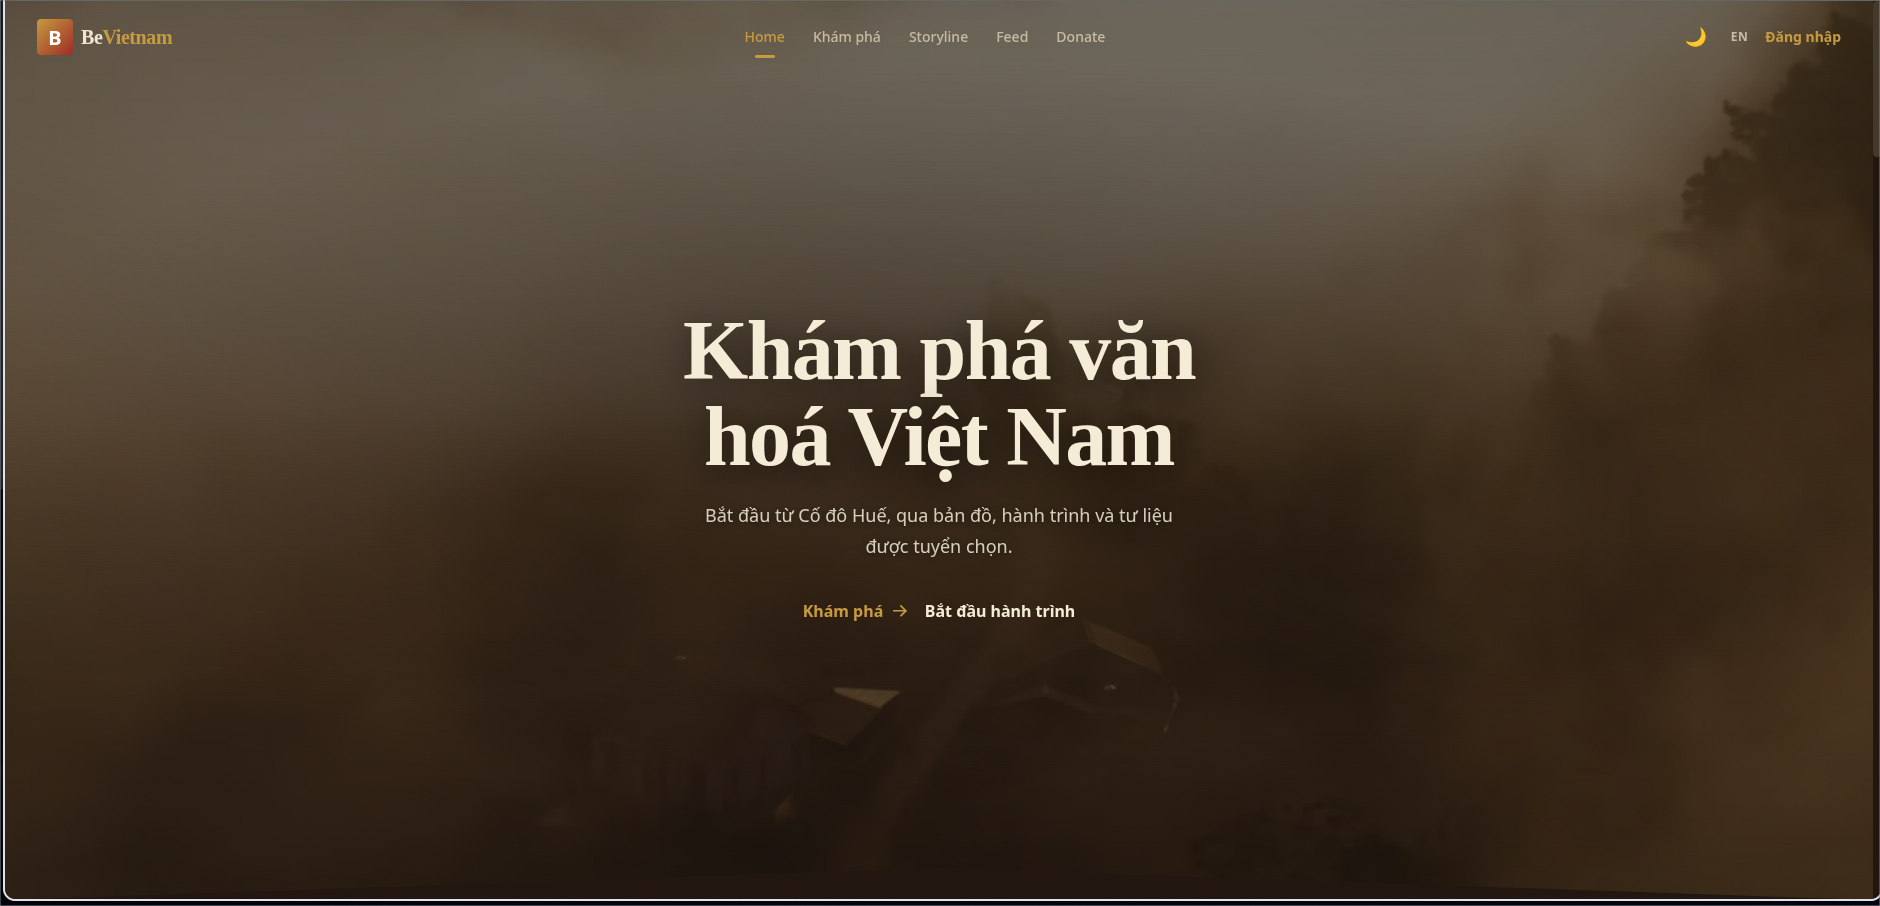
\includegraphics[width=\linewidth]{../report/images/bevietnam_homepage.jpg}}
    {\fcolorbox{UFTgray!50}{UFTgray!12}{\parbox[c][4.6cm][c]{\linewidth}{\centering\itshape\color{UFTgray}bevietnam\_homepage.jpg\\(thêm vào report/images/)}}}
  \end{center}
  \column{0.30\textwidth}
  \kw{Next.js (Azure)}\\[5pt]
  \kw{Feed gợi ý}\\[5pt]
  \kw{Bubble map}\\[5pt]
  \kw{Storyline}\\[5pt]
  \kw{Song ngữ}
  \end{columns}
\end{frame}

% ── Slide 12a2: Mobile app ───────────────────────────────────────────
\begin{frame}{Sản phẩm --- Mobile App (Android)}
  \begin{center}
  \mobshot{mobile_login.jpg}{login}\hfill
  \mobshot{mobile_map.jpg}{map}\hfill
  \mobshot{mobile_storyline.jpg}{storyline}\hfill
  \mobshot{mobile_post.jpg}{post}
  \end{center}
  \vspace{1mm}
  \begin{center}\scriptsize
  \kw{Đăng nhập} \quad \kw{Bản đồ thời gian thực} \quad \kw{Storyline} \quad \kw{Feed} \quad --- Jetpack Compose
  \end{center}
\end{frame}

% ── Slide 12b: vLLM serving terminal ─────────────────────────────────
\begin{frame}{vLLM serving --- terminal thực tế}
  \begin{center}
  \IfFileExists{../report/images/vllm.png}
    {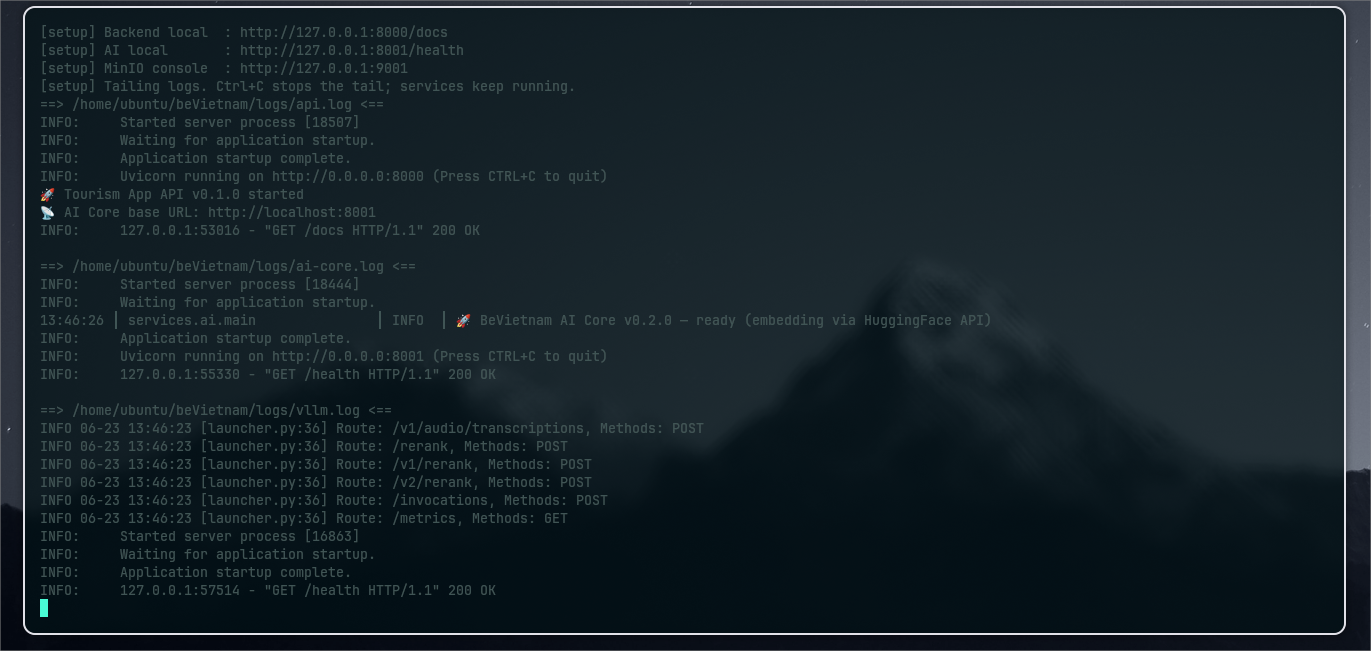
\includegraphics[width=0.92\textwidth]{../report/images/vllm.png}}
    {\fcolorbox{UFTgray!50}{UFTgray!12}{\parbox[c][4cm][c]{0.85\textwidth}{\centering\itshape\color{UFTgray}vllm.png\\(thêm screenshot terminal vLLM)}}}
  \end{center}
  \vspace{1mm}
  \begin{center}\scriptsize
  \kw{1 card L40 đủ cho 7B + KV-cache} \quad \kw{2 ảnh / request} \quad \kw{phục vụ /verify-capture}
  \end{center}
\end{frame}

% ── Slide 13: Testing / Status ───────────────────────────────────────
\begin{frame}{Kiểm thử \& trạng thái pilot}
  \begin{columns}[T]
  \column{0.5\textwidth}
  \footnotesize
  \begin{tabular}{@{}ll@{}}
  \toprule
  \textbf{Kiểm thử} & \textbf{Kết quả} \\
  \midrule
  /places/nearby (HCMC) & 200 POI, 5 nhóm \\
  /question-pool & 133 nhiệm vụ \\
  Capture (ảnh sai) & rejected/needs\_review \\
  Build web + mobile & OK \\
  \bottomrule
  \end{tabular}
  \column{0.5\textwidth}
  \kw{Huế pilot}\\[4pt]
  \kw{Web + Mobile + AI Core + vLLM chạy thật}\\[4pt]
  \scriptsize \textit{Hạn chế hiện tại:} traffic/crowd mô phỏng; xác minh ảnh cần duyệt tay ở vùng nghi ngờ.
  \end{columns}
\end{frame}

% ── Slide 14: Conclusion ─────────────────────────────────────────────
\begin{frame}{Kết luận \& hướng phát triển}
  \begin{columns}[T]
  \column{0.5\textwidth}
  \textbf{Đã làm}
  \begin{itemize}\footnotesize
    \item Gợi ý ngữ cảnh + giải thích được
    \item Bản đồ POI thời gian thực
    \item Storyline gắn hành động thực địa
    \item Xác minh ảnh bằng VLM tự host
  \end{itemize}
  \column{0.5\textwidth}
  \textbf{Tiếp theo}
  \begin{itemize}\footnotesize
    \item Tín hiệu traffic/crowd thật
    \item Mở rộng ngoài Huế
    \item Moderation + admin
    \item Cá nhân hóa sâu hơn
  \end{itemize}
  \end{columns}
  \vfill
  \begin{center}\large\color{UFTblue}\textbf{Cảm ơn --- Q\&A}\end{center}
\end{frame}

\end{document}
